
%%% Preamble
\documentclass[paper=a4, fontsize=11pt]{scrartcl}
\usepackage[utf8x]{inputenc}
%\usepackage[T1]{fontenc}
\usepackage[brazilian]{babel}															% English language/hyphenation
\usepackage[protrusion=true,expansion=true]{microtype}	
\usepackage{amsmath,amsfonts,amsthm} % Math packages
\usepackage{graphicx}	
\usepackage{url}
\usepackage{caption}
\usepackage{subcaption}
\usepackage{float}
\floatplacement{figure}{H}


%%% Custom sectioning
\usepackage{sectsty}
\allsectionsfont{\centering \normalfont\scshape}


%%% Custom headers/footers (fancyhdr package)
\usepackage{fancyhdr}
\pagestyle{fancyplain}
\fancyhead{}											% No page header
\fancyfoot[L]{}											% Empty 
\fancyfoot[C]{}											% Empty
\fancyfoot[R]{\thepage}									% Pagenumbering
\renewcommand{\headrulewidth}{0pt}			% Remove header underlines
\renewcommand{\footrulewidth}{0pt}				% Remove footer underlines
\setlength{\headheight}{13.6pt}

\graphicspath{{img/}}

%%% Equation and float numbering
\numberwithin{equation}{section}		% Equationnumbering: section.eq#
\numberwithin{figure}{section}			% Figurenumbering: section.fig#
\numberwithin{table}{section}				% Tablenumbering: section.tab#


%%% Maketitle metadata
\newcommand{\horrule}[1]{\rule{\linewidth}{#1}} 	% Horizontal rule

\title{
		%\vspace{-1in} 	
		\usefont{OT1}{bch}{b}{n}
		\normalfont \normalsize \textsc{UFMG - Departamento de Ciência da Computação} \\ [25pt]
		\horrule{0.5pt} \\[0.4cm]
		\huge Coletor para a Web Brasileira \\
		\horrule{2pt} \\[0.5cm]
}
\author{
		\normalfont 								\normalsize
        Gabriel Miranda Pedrosa\\[-3pt]		\normalsize
        %\today
}
%\date{}


%%% Begin document
\begin{document}
\maketitle
\section{Introdução}
O desenvolvimento da rede mundial de computadores criou a necessidade de recuperar as informações nela contida através de máquinas de busca. Uma das etapas da construção de uma máquina de busca da Web é a coleta de suas páginas.

O primeiro trabalho da disciplina de Recuperação da Informação tem como objetivo a construção de um coletor da Web brasileira que seja horizontal, ou seja, que foque em buscar a maior quantidade possível de domínios. O coletor deve ser respeitoso com os domínios visitados, não sobrecarregando servidores. Instruções dadas pelos sítios para coleta devem ser respeitadas.

\section{O Coletor}
A coleta das páginas começa em um determinado conjunto de páginas semente. Através dos \textit{links} presentes em cada uma dessas páginas, a navegação pela rede de computadores continua, coletando páginas e outros endereços nelas presentes. O carregamento das páginas e extração de \textit{links} foi feita através da versão gratuita da biblioteca Chilkat Spider \footnote{Disponível em \url{https://www.chilkatsoft.com/chilkatLinux.asp}}.

Para cumprir os requerimentos de coleta horizontal, o coletor foi projetado com um escalonador de páginas para coleta. O escalonador define a próxima URL a ser coletada levando em consideração a profundidade das URLs e a penalidade de seus domínios no momento que as URLs são observadas, de forma que, quanto menos profunda a URL e menos links para um domínio a fila possui, maior a prioridade da URL para coleta. A profundidade é calculada contando quantas barras (o caractere '/') a URL possui, desconsiderando as barras da definição do protocolo. O objetivo é favorecer páginas que estejam mais próximas da raiz do sítio.

Como o objetivo é construir um coletor da Web brasileira, as URLs foram filtradas para que somente fossem coletadas páginas do domínio ``.br", com exceção de páginas brasileiras conhecidas que não estão no domínio, como \textit{globo.com}, \textit{r7.com}, \textit{ingresso.com} e \textit{amocinema.com}. Outras URLs também eram excluídas da coleta, como encurtadores de link, botões de compartilhamento de rede social, URLs construídas em tempo de execução do site através de \textit{templates} Javascript, e URLs para validadores CSS.

Alguns processamentos são feitos nas URLs antes de serem adicionadas ao escalonador, como transformação de todas as letras para minúsculo, remoção de barras extras no trecho de definição de protocolo, remoção de espaços e final da URL quando indica raiz de uma pasta ('/', '/index.html', '/index.php', etc). Se, mesmo com essas correções, ainda não for possível extrair domínio e subdomínio da URL, ela não é considerada.

A preservação dos servidores é garantida no escalonador, que verifica se o último acesso ao domínio da página mais indicada para ser coletada foi muito recente, menos de 30 segundos atrás. Se for o caso, a penalidade do domínio é atualizada e a busca por uma página adequada continua. Quando a busca termina, as páginas extraídas do escalonador que não puderam ser coletadas são inseridas novamente com penalidades atualizadas.

Para garantir melhor desempenho do escalonador, sua implementação foi feita usando a estrutura de dados Min-max heap, que permite saber, em tempo constante, o menor e o maior elemento da fila, enquanto remoções e inserções são feitas em tempo logarítmico no número de entradas. Essa funcionalidade é importante por permitir a definição rápida não só da próxima página a ser coletada mas também qual página deve sair da fila de prioridades para dar lugar a uma nova, caso a fila exceda seus limites de espaço.

A coleta das páginas é feita de forma concorrente, disparando \textit{threads} que requerem páginas do escalonador e as coletam enquanto o número de páginas coletadas for inferior ao requerido. O conteúdo das páginas é agregado em um \textit{buffer} antes de ser salvo em disco. 

\paragraph{\textbf{ANÁLISE DE COMPLEXIDADE}} As duas operações principais do coletor são a inserção de URL nova no escalonador e a escolha da próxima a ser coletada. O tamanho do endereço da página é desconsiderado na análise de complexidade por ser muito menor que o número de páginas no escalonador, indicado nas análises posteriores como $N$.

A inserção de nova página formata a URL, verifica em uma tabela hash se já foi adicionada anteriormente, verifica em outra tabela hash as informações de acesso ao domínio da página, atualiza esses valores e adiciona a página ao escalonador. Todas as operações são $O(1)$, com exceção da última que é logarítimica no número de elementos do escalonador. A inserção tem, portanto, complexidade de tempo $O(\log N)$. 

A escolha da próxima página a ser coletada remove páginas do topo da heap enquanto não encontra uma que possa ser coletada. No caso médio, a escolha tem custo $O(\log N)$. No pior caso, entretanto, o escalonador remove todas as páginas da heap para depois adicioná-las novamente, o que tem custo $O(N * \log N)$.

Com relação a análise de complexidade de espaço, o coletor projetado tem complexidade $O(N) + O(C)$, sendo $C$ o número de páginas já vistas. Além do heap do escalonador, são armazenadas todos os endereços de páginas já vistas em uma tabela hash, assim como informações sobre seus domínios.

\section{Experimentos}
Idealmente, o coletor deve progredir de forma constante e seu desempenho não deve cair ao aumentar o número de páginas disponíveis no escalonador. A quantidade de \textit{threads} disparadas deve ser adequada para o ambiente de execução, não causando \textit{thrashing} do sistema durante a execução. 

Para verificar esses pontos para o coletor projetado, foram realizados alguns experimentos com velocidade de coleta, banda utilizada e número adequado de \textit{threads}. Os testes foram realizados em um computador disponível no CRC, cujas configurações são:
\begin{itemize}
	\item Intel Core 2 Duo E7500 @ 2.93GHz
	\item 4GB de RAM
	\item Ubuntu 14.04.5 LTS
	\item Velocidade da internet durante teste:
		\begin{itemize}
			\item Download: 3.45 Mbit/s
			\item Upload: 3.20 Mbit/s
		\end{itemize}
\end{itemize}

Informações sobre velocidade de escrita no disco não foram recuperadas. Porém, como a escrita das páginas em disco é feita somente quando 300 páginas são coletadas, a velocidade de escrita não atrapalhará tanto o desempenho do coletor.

Por causa da limitação de memória RAM, o tamanho máximo do escalonador foi fixado em 1 milhão. Quando o tamanho era excedido, a página com menor preferência era descartada para dar lugar à nova. 

\paragraph{\textbf{\textit{THREADS}}} O desempenho do coletor foi testado com 20, 50, 80, 110 e 130 \textit{threads}, fixando o número de páginas coletadas em 5 mil. O resultado pode ser observado na Figura \ref{fig:threads}, que indica que o desempenho foi máximo com 110 \textit{threads}. Com 130, houve perda de velocidade de coleta possivelmente ocasionada por \textit{thrashing} do sistema ou uso da banda além do adequado.

\paragraph{\textbf{TEMPO}} O número de \textit{threads} foi fixado em 110, já que o experimento anterior indicou que essa era uma boa quantidade para o ambiente de execução, e o número de páginas a serem coletadas em 1 milhão. O objetivo do experimento é verificar se o desempenho do coletor cai quando o número de páginas coletadas cresce. O coletor demorou 5 horas e 17 minutos. A Figura \ref{fig:tempo} mostra que o progresso da coleta foi constante.

\paragraph{\textbf{BANDA}} O experimento de banda gasta registrou quantos bytes de páginas foram salvos em cada segundo e determinou que, para aquele instante, a banda média é a média de bytes salvos nos 20 segundos anteriores. A Figura \ref{fig:banda} apresenta a variação de banda utilizada no decorrer da coleta.

\paragraph{\textbf{QUALIDADE}} A análise de qualidade da coleta visa confirmar o comportamento esperado de coleta horizontal, que deve priorizar a variedade 
de domínios no lugar de coletar diversas páginas de um somente. Os domínios atingidos pelo coletor quando coletadas 1 milhão de páginas somaram 153 mil. O número de páginas coletadas por domínio variou de 1 a 14 páginas, com mediana 7 e média 6,5. A distribuição pode ser melhor visualizada na Figura \ref{fig:distribuicao}.

A busca não foi extremamente horizontal, visto que o coletor visitou um grupo de páginas da maior parte dos domínios. Mas, considerando que o grupo foi pequeno e que as informações de páginas de dentro de um mesmo domínio são importantes, considero que a implementação do coletor foi correta.

\section{Melhorias}
Muitas URLs encontradas eram malformadas, o que quebrou a execução do coletor diversas vezes na etapa de implementação. Algumas ações foram feitas para que as URLs fossem corrigidas, porém, os erros são muito imprevisíveis. O ideal é, portanto, que fosse feita uma validação da URL através de expressões regulares, por exemplo, antes de ser adicionada ao coletor, descartando as malformadas.

Os parâmetros passados ao coletor permitem que o usuário regule o consumo de banda indiretamente ao diminuir o número de \textit{threads} disparadas. Porém, é necessária experimentação. Uma melhoria possível seria adaptar o ritmo da coleta às necessidades ou limitações do ambiente do usuário, fornecendo o gasto de banda máximo como parâmetro.

\begin{figure}
  \caption{Velocidade de coleta com diferentes números de \textit{threads}}
  \label{fig:threads}
  \centering
    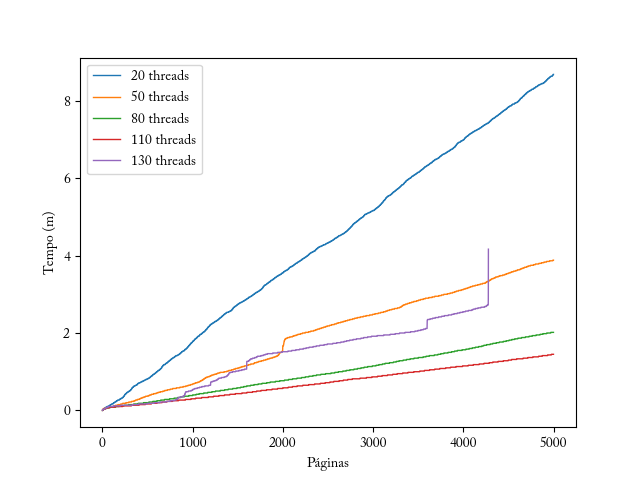
\includegraphics[width=1\textwidth]{threads}
\end{figure}

\begin{figure}
  \caption{Progresso da coleta em função do tempo}
  \label{fig:tempo}
  \centering
    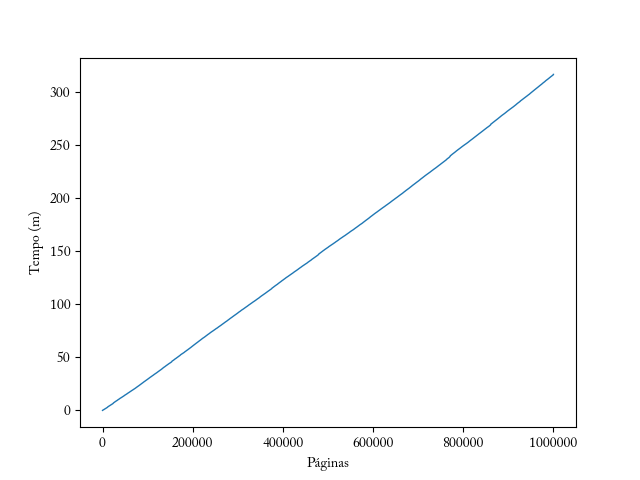
\includegraphics[width=1\textwidth]{tempo}
\end{figure}

\begin{figure}
  \caption{Largura de banda média utilizada durante a coleta}
  \label{fig:banda}
  \centering
    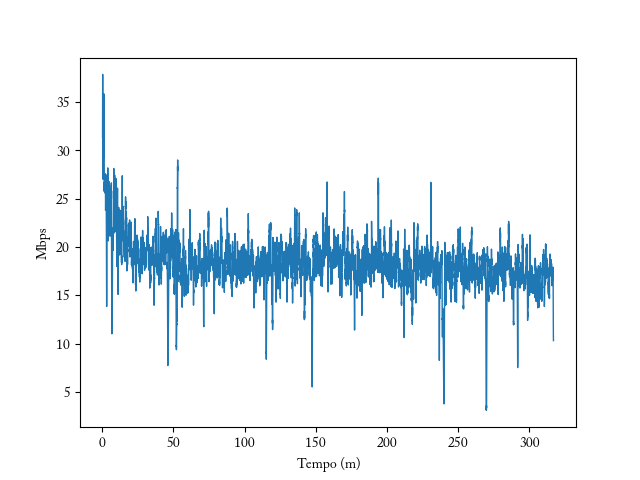
\includegraphics[width=1\textwidth]{banda}
\end{figure}


\begin{figure}
  \caption{Distribuição de páginas coletadas por domínio}
  \label{fig:distribuicao}
  \centering
    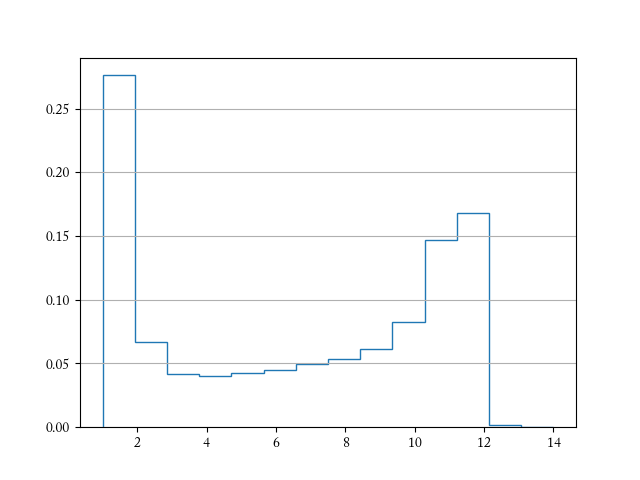
\includegraphics[width=1\textwidth]{por-dominio}
\end{figure}


%%% End document
\end{document}